\section{Background}
{\color{red}---Catchy first sentence.}\newline
\textit{Machine learning} aims to infer generally valid relationships from a finite set of training data and apply those learned relations to new data \cite{domingos2012few} \cite{kotsiantis2007supervised}. While some problems can be solved by manually encoding explicit rules, others require a different approach as explicit decision-making does not deliver highly accurate results \cite{burrell2016machine}. Determining a student's grade in a multiple choice test can be solved by explicitly encoding mathematical rules, yet deciding whether the tonality of a text is positive or negative needs more than a simple rule set to function accurately \cite{melville2009sentiment}. The datasets needed to train machine learning models are often large and represented in a high-dimensional feature space, which makes it impossible for a human to carry out the learning task like a machine can. However, machines can be used to extend the cognitive capabilities of humans when working together on those learning tasks. \cite{ventocilla2018taxonomy} describes the fruitful collaboration between human and machine as \textit{augmented intelligence}, pointing at the positive aspect of machine learning support.\newline
{\color{red}---Narrowing topic to decision-making and discriminative algorithms and define "decision" as output from ML systems}


%------------------------------------------------------------------
\subsection{Interpretability in AI}
Humans cooperating with machines need to understand the principles of the method that is employed - a property referred to as \textit{transparency} \cite{kotsiantis2007supervised}. \textit{Opacity}, the direct opposite of transparency \cite{lipton2016mythos}, is a major problem for augmented intelligence. Although opacity can be used voluntarily as a means to self-protection and censorship, it also arises involuntarily due to missing technical expertise and failed human intuition and cognitive abilities \cite{burrell2016machine}.\newline
On the application-side of machine learning systems, the question of transparency brings up the notion of \textit{interpretability}. Interpretability refers to how well a ``typical classifier generated by a learning algorithm" can be understood \cite{kotsiantis2007supervised}, as compared to the theoretical principle of the method. That is, an interpretable machine learning system is either inherently interpretable, meaning that its operations and result patterns can be understood by a human \cite{biran2017explanation} \cite{ventocilla2018taxonomy}, or it is capable of generating descriptions understandable to humans \cite{gilpin2018explaining}. It is also possible to equip a system retrospectively with interpretability by adding a proxy model capable of mirroring the original system's behaviour while being comprehensible for humans \cite{guidotti2018survey}. Using an interpretable system as a human means being enabled to make inferences about underlying data \cite{ventocilla2018taxonomy}.\newline
\cite{guidotti2018survey} assigns ten desired dimensions to interpretable machine learning systems:
\begin{itemize}
	\item \textit{Scope}: Global interpretability (understanding the model and operations) and local interpretability (understanding what brought about a single decision)
	\item \textit{Timing}: Time scope available in the application use case for a target user to understand 
	\item \textit{Prior knowledge}: Level of expertise of target user
	\item \textit{Dimensionality}: Size of the model and the data
	\item \textit{Accuracy}: Target accuracy of the system while maintaining interpretability
	\item \textit{Fidelity}: Accuracy of explanation vs. accuracy of model
	\item \textit{Fairness}: Robustness against automated discrimination and ethically challenging biases in data
	\item \textit{Privacy}: Protection of sensible and personal data
	\item \textit{Monotonicity}: Level of monotonicity in relations of input and output (human intuition is largely monotonic)
	\item \textit{Usability}: Efficiency, effectiveness, and joy of use
\end{itemize}
In the context of interpretability for machine learning systems, the terms \textit{understandability}, \textit{comprehensibility}, \textit{explainability}, and \textit{justification} are often mentioned in literature. In this paper, we adopt the definition of \cite{ruping2006learning}. \textit{Understandability}, \textit{accuracy} of the explanation, and \textit{efficiency} of the explanation together form \textit{interpretability}. \textit{Explainability} is a synonym of \textit{comprehensibility} \cite{weihs2003combining}, which is also synonymic to \textit{understandability} \cite{bibal2016interpretability} and therefore an aspect of interpretability, showing the reasons for the system's behaviour \cite{gilpin2018explaining}. Figure \ref{fig:definitions} gives an overview over these terms. Finally, \textit{justification} refers to the evidence for why a decision is correct, which does not necessarily include the underlying reasons and causes \cite{biran2017explanation}.\newline
\begin{figure} [h]
	\centering
	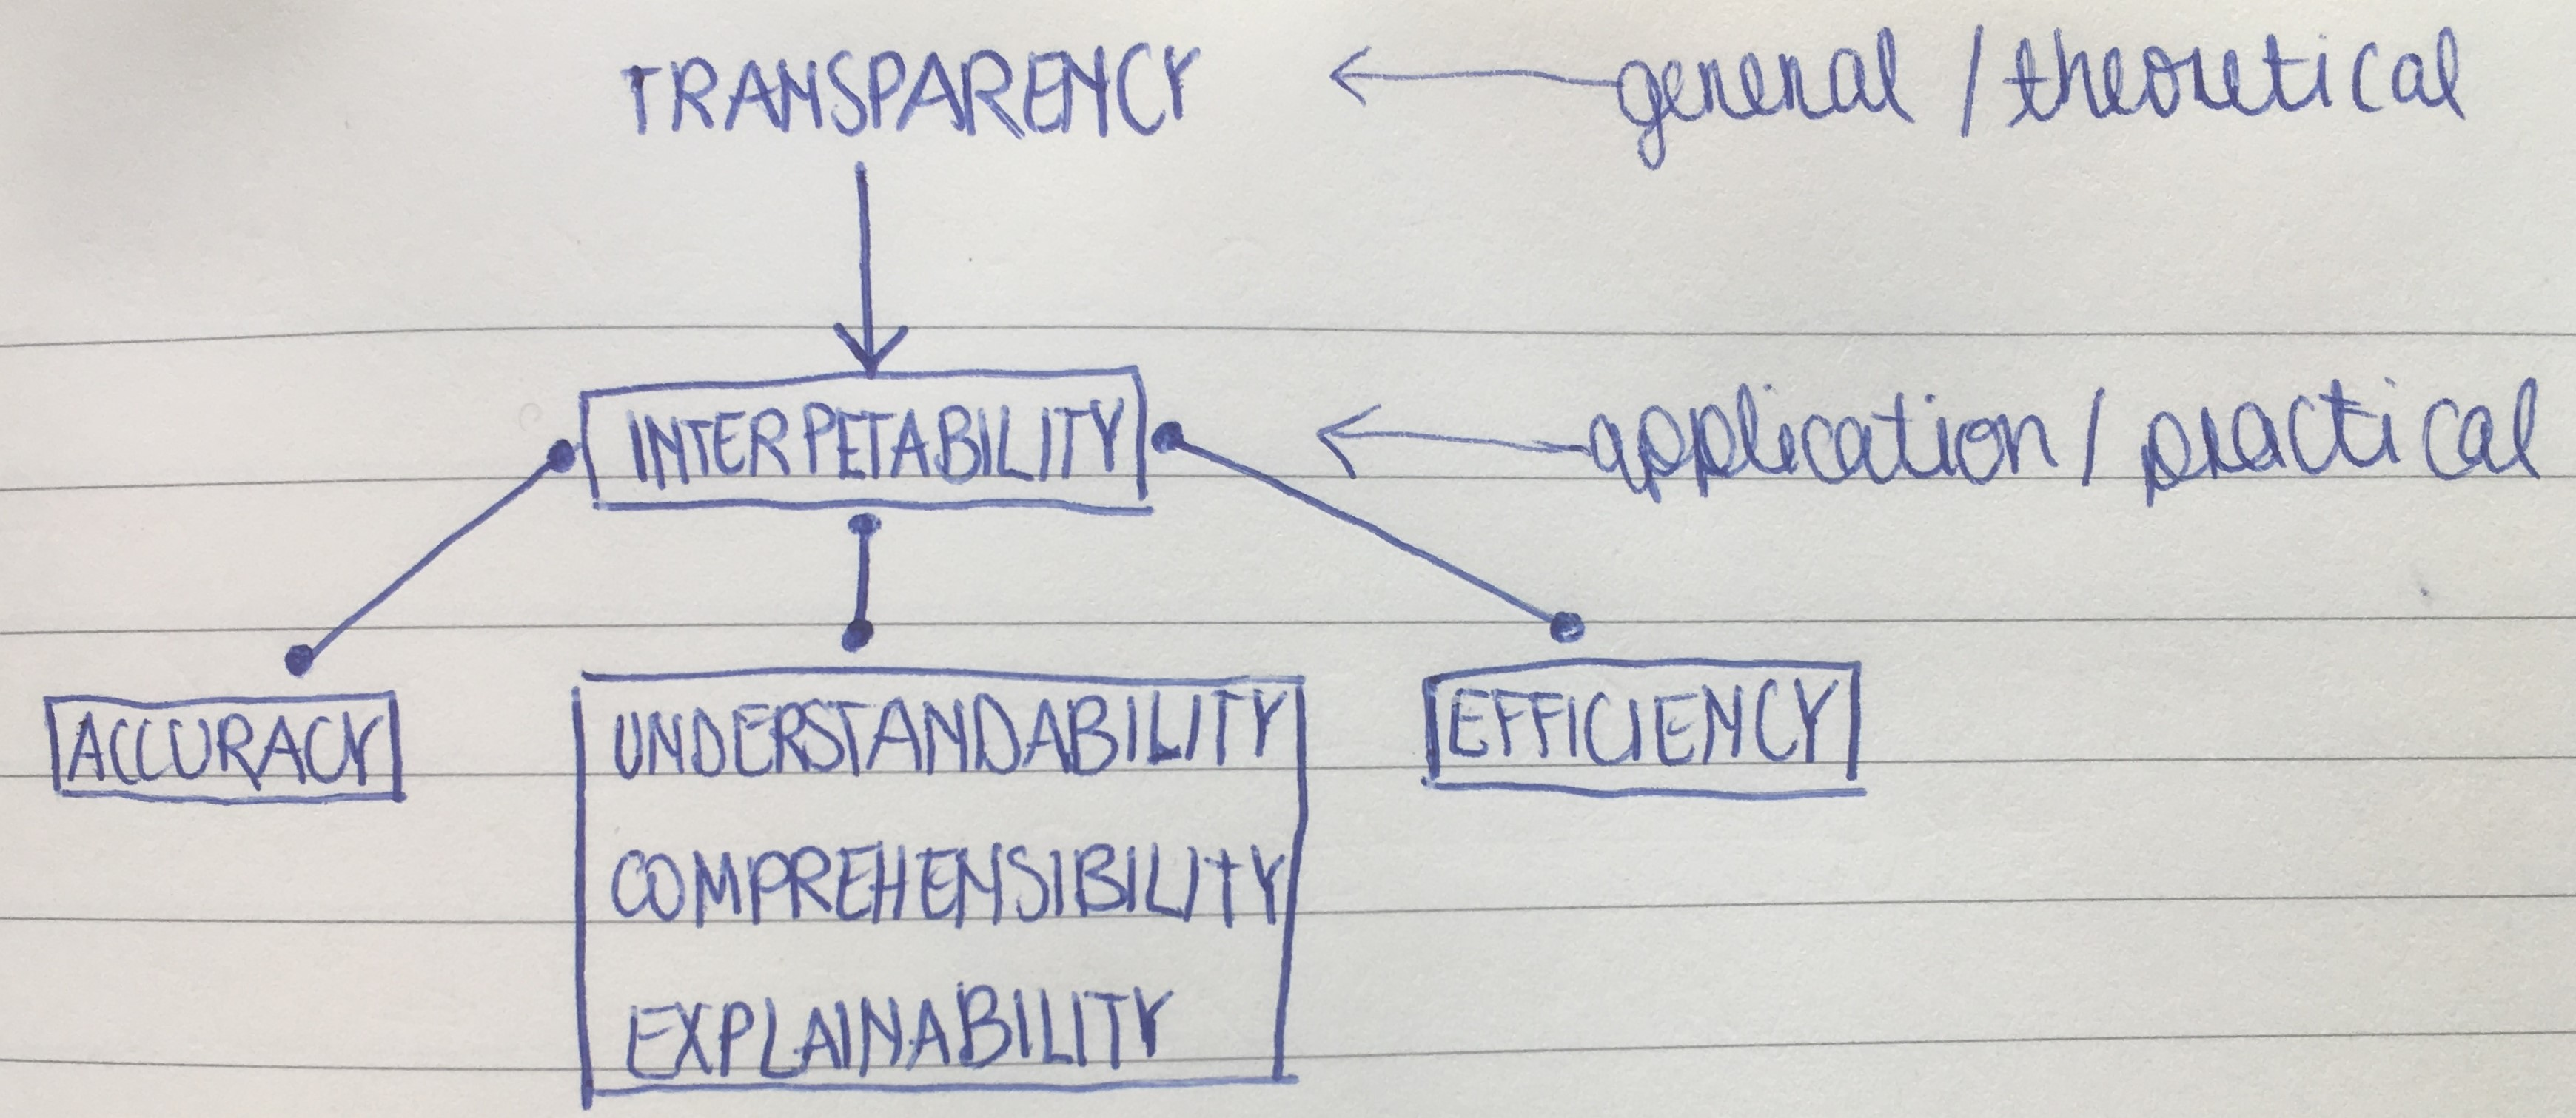
\includegraphics[width=0.7\linewidth]{img/definitions}
	\caption{Relation of terms connected to interpretability}
	\label{fig:definitions}
\end{figure}
If the human cognition is augmented by a machine learning system, talking about interpretability should also include discussing the interpretability of the human in the loop. \cite{lipton2016mythos} argues that human behaviour is often mistakenly identified as interpretable because humans can explain their actions and beliefs. Yet the actual operations of the human brain remain opaque, which contradicts the concept of interpretability \cite{lipton2016mythos}. If human interpretability is taken as a point of reference for the discussion of algorithmic interpretability, \cite{lipton2016mythos}'s argument should be taken into account. Human interpretability, however, is not the focus of this paper and will therefore not be discussed in more detail here.\newline





%------------------------------------------------------------------
\subsection{Need for Explainability in AI}
\label{subsec:explainability}
A subfield of artificial intelligence research revolves solely around the explainability of intelligent systems: \textit{xAI}, explainable artificial intelligence, for the purpose of enabling communication with agents about their reasoning \cite{hendricks2018generating}. xAI systems face a trade-off challenge: Their explanation has to be complete and interpretable at the same time \cite{gilpin2018explaining}. The attention span and cognitive abilities of humans therefore become an important factor to consider in the design of a xAI systemm \cite{kulesza2013too}. Furthermore, the goal of explaining the system is twofold: create actual knowledge and convince the user that the knowledge is sound and complete. Actual understanding and perceived understanding however do not always go hand in hand: Persuasive systems can convince the user without creating actual transparency \cite{gilpin2018explaining}. The persuasiveness of an explanation is uncoupled from the actual information content of an explanation \cite{biran2017explanation} and needs to be taken into account in user studies. As users can only report on their perception of the explanation, an objective measure to evaluate the fidelity of an explanation is needed. High-fidelity (also called descriptive) explanations are faithful, in that they represent truthful information about the underlying machine learning model \cite{herman2017promise}. Persuasive explanations, on the opposite, are less faithful to the underlying model, yet open up possibilities for abstraction, simplification, analogies, and other stylistic devices for communication. \cite{herman2017promise} notes a dilemma in explanation fidelity: ``This freedom permits explanations better tailored to human cognitive function, making them more functionally interpretable", but ``descriptive explanations best satisfy the ethical goal of transparency". The xAI practitioner therefore needs to consider a tradeoff between fidelity and interpretability. \newline 
Besides low-fidelity persuasiveness, badly designed explanations likewise ``provide an understanding that is at best incomplete and at worst false reassurance" \cite{burrell2016machine}. Therefore, not only possible explanations for white box (inherently interpretable) and black box (inherently non-interpretable) systems need to be examined, but also the (visual) design and communication of explanations \cite{guidotti2018survey}. \newline
In recent years, machine learning algorithms employed in the wild show a trend towards increasing accuracy but also increasing complexity. In general, the higher the accuracy and complexity, the lower the explainability \cite{richardson2018survey} \cite{chen2018learning} in machine learning. However, users do not necessarily perceive systems with simple explanations as more understandable \cite{allahyari2011user}. The authors of the user study in \cite{allahyari2011user} hypothesise that users detect missing information in simple explanations, which in turn leads to the perception of incomprehensibility. \cite{van2018contrastive} examined user preferences in more detail and concluded that users overall preferred more soundness and completeness over simplicity, as well as global explanations over local explanations.\newline
Humans involved in the explanation process are not only users, but also domain experts and engineers during the design and training phase. As explanations are user-dependent (not monolithic) \cite{preece2018asking}, the design and evaluation of explanation needs to be conducted in reference to the target users. Including experts in the modelling and training process is not only a way to integrate expert knowledge that is otherwise difficult to model, but can also increase user trust \cite{ventocilla2018taxonomy}. \cite{liu2017towards} call the situation where a human expert works alongside the machine learning system to improve it ``mixed initiative guidance". \newline

\subsubsection{Explanation Goals}
\label{subsubsec:Explanation Goals}
Machine learning systems are able to achieve high accuracy on classification tasks, for example in information retrieval, data mining, speech recognition, and computer graphics \cite{liu2017towards}. Explainability is a means to ensure that machine learning systems are not only right in a high number of cases, but right for the right reasons \cite{preece2018asking}. High accuracy does not necessarily mean that correct generalisations were learned from the dataset or that no biases were present in the data.\newline
The need for interpretability is dependent on the role of the explanation user and the severity of the consequences of the classification result and possible errors. Since explanations are not monolithic, i.e. have to be adapted to the target user's level of expertise, preferences for explanation types, and cognitive capabilities, the need for interpretability is also dependent on the targeted audience. Furthermore, different users can have different data access rights and have different goals to achieve in their interaction with the system \cite{vorm2018assessing}. While an engineer could be interested in technical details, a bank employee assessing loan credibility could be interested in similar cases and relevant characteristics of a single decision case. \cite{richardson2018survey} separates a general need for interpretability into three categories:
\begin{itemize}
	\item \textbf{no need} for interpretability if no consequences arise from faulty decisions
	\item interpretability is \textbf{beneficial} if consequences for individuals arise from faulty decisions
	\item interpretability is \textbf{critical} if serious consequences arise from faulty decisions
\end{itemize}
The three classes of interpretability needs give an overview about possible consequences, yet are too general to serve as guideline for practitioners. More details about decisive factors are needed.\newline
For users of an automatic decision system, having insights into the system functioning and decision process increases trust \cite{preece2018asking} \cite{diakopoulos2016accountability} \cite{biran2017explanation} \cite{cramer2008effects} \cite{vorm2018assessing}, even in critical decisions such as medical diagnosis \cite{allahyari2011user}. The level of trust should be in relation to the soundness and completeness of an explanation. Having too much or too little trust in a system can hinder fruitful interaction between the user and the system \cite{preece2018asking} \cite{richardson2018survey} \cite{van2018contrastive} \cite{ribeiro2016should}. Other positive effects on users are satisfaction and acceptance \cite{biran2017explanation} \cite{cramer2008effects} \cite{vorm2018assessing} as well as the ability to predict the system's performance correctly \cite{biran2017explanation}.\newline
\cite{liu2017towards} identifies three goals of explanability in machine learning:
\begin{itemize}
	\item \textit{Understanding and reassurance}: right for the right reasons
	\item \textit{Diagnosis}: analysis of errors, unacceptable performance, or behaviour
	\item \textit{Refinement}: improving robustness and performance
\end{itemize}
From the point of view of engineers and experts, explanations help to design, debug, and improve an automatic decision system \cite{preece2018asking}. Explanations facilitate the identification of unintuitive, systematic errors \cite{gilpin2018explaining} \cite{ribeiro2016should} in the design and redundantise time-consuming trial-and-error procedures for parameter optimisation \cite{liu2017towards}. Unethical biases in training data leading to automated discrimination \cite{diakopoulos2016accountability} can be identified and examined via explanations \cite{gilpin2018explaining} \cite{richardson2018survey} \cite{ribeiro2016should}. Ultimately, the early identification of errors avoids costly errors in high-risk domains \cite{diakopoulos2016accountability} \cite{bibal2016interpretability} \cite{van2018contrastive} and ensures human safety in safety-critical tasks \cite{gilpin2018explaining} \cite{richardson2018survey}.\newline
Besides helping users and engineers, explanations also serve general goals of protection, conformity, and knowledge management. Criminals or hackers that aim to disturb the system or take advantage of it can make imperceptible changes to the input data or model at hidden levels. Having a system capable of explaining its behaviour and inner structure helps to identify unwanted alterations \cite{gilpin2018explaining}. With the European General Data Prodection Regulation (GDPR) put into place in 2018, a debate on a \textit{right to explanation} started, which will be discussed in the following section. Although the specific implications of the right to explanation remain unclear, it should still be noted that designing interpretability follows up on that regulation \cite{goodman16eu} \cite{gilpin2018explaining} \cite{bibal2016interpretability}. Finally, the most general goal of implementing explanations for automatic decision systems is the opening and accessibility of a knowledge source \cite{bibal2016interpretability} \cite{richardson2018survey}. The relations derived by a machine learner (stored in the model) can deliver relevant knowledge about the data at hand.\newline


\subsubsection{Regulations and Accountability}
The General Data Protection Regulation (GDPR) is a European law dealing with the processing of personal data within the European Economic Area (EEA, includes also all countries of the EU). The law holds for all companies within the EEA, companies with subsidiaries in the EEA, and any company processing personal data of a citizen of the EEA. In this context, ``processing" does not only relate to automatic systems but also spans to manual processing of personal data \cite{goodman16eu}. The GDPR defines personal data as data relating to an identifiable natural person, i.e. data that can be used to identify a person {\color{red}[REF TO LAW TEXT]}. Names, location data, or personal identification numbers are all examples of personal data that falls under the GDPR. \cite{goodman16eu} identifies two consequences of the GDPR: the legal right to non-discrimination, and a right to explanation.\newline
Algorithmic decisions must not be based on sensitive, personal data (GDPR article 22 paragraph 4) that are nowadays used to identify groups of people with similar characteristics, such as ethnicity, religion, gender, disability, sexuality, and more \cite{diakopoulos2016accountability}. Sensitive information can, however, correlate with non-sensitive data. Real-life data almost always reflects a society's structures and biases - explicitly through sensitive information, or implicitly via dependent information. As the task of classification means separating single instances into groups based on the available data, the biases are recovered in the model \cite{goodman16eu}. A guarantee non-discrimination is therefore difficult to achieve. The GDPR does not specify whether only sensitive data or also correlated variables have to be considered when following the law. \cite{goodman16eu} identifies both interpretations as possible.\newline
While article 13 of the GDPR specifies a right to obtain information about one's personal information and the processing of that personal information, it assures ``meaningful information about the logic involved" in profiling without further defining meaningfulness. Based on the ambiguity of ``meaningful", several interpretations exist, ranging from denial of the ``right to explanation" \cite{wachter2017right} to a positive interpretation \cite{selbst2017meaningful}. In summary, precedents are needed to clarify the boundaries of the law.\newline
Besides legal regulations, ethical considerations also play a role in augmented intelligence. Accountability is the ethical value of acknowledging responsibility for decisions and actions towards another party \cite{baldoni2016computational}. It is an inherent factor in human-human interaction; artificial intelligence employed to interact with humans or collaborate with humans in augmented intelligence settings therefore bring about the challenge of ``computational accountability" \cite{baldoni2016computational}. It is important to note that accountability is not a general issue in the digital world: For something to be held accountable of its own decisions or actions, it needs to act autonomously {\color{red}[REF WENT MISSING; CHECK AGAIN IN NOTES]}. In order to determine autonomy of an algorithm and work towards accountability, \cite{diakopoulos2016accountability} suggests to disclose the following information for machine learning systems: 
\begin{itemize}
	\item \textit{Human involvement}: who controls the algorithm, who designed it etc., leading to control through social pressure
	\item \textit{Data statistics}: accuracy, completeness, uncertainty, representativeness, labelling \& collection process, preprocessing of data
	\item \textit{Model}: input, weights, parameters, hidden information
	\item \textit{Inferencing}: covariance matrix to estimate risk, prevention measures for known errors, confidence score 
	\item \textit{Algorithmic presence}: visibility, filtering, reach of algorithm
\end{itemize}
\cite{baldoni2016computational} argues that causality is a necessary prerequisite for accountability. Machine learning algorithms often learn statistical relations between input features, which at best leads to probabilistic causality, but not certainly to deterministic causality. Whether an automatic decision system itself can be held accountable for its decisions is therefore debatable.





%------------------------------------------------------------------
\subsubsection{Application Areas}
Artificial intelligence and machine learning algorithms are nowadays employed in a variety of areas. As described in \ref{subsubsec:Explanation Goals}, the need for interpretability depends on the potential consequences of the decisions made by an automatic system. \cite{burrell2016machine} summarises the application area as all systems with ``socially consequential mechanisms of classification and ranking", pointing in particular to the consequences for humans. A similar view is expressed in \cite{poursabzi2017manipulating} and \cite{ribeiro2016should}, while \cite{guidotti2018survey} restricts the application areas in need for interpretability to those that process sensitive, i.e. personal data. In more detail, the following areas in need of interpretable intelligent systems are mentioned in literature:
\begin{itemize}
	\item \textit{Societal safety}: criminal justice [52] [19], terrorism detection [24]	
	\item \textit{Processing sensitive data}: banking, e.g. loans [52] [6] [19] [33] [36], medicine \& health data [52] [3] [1] [15] [19] [16] [24], insurances [3] [33] [36], navigation [1]
	\item \textit{Physical safety}: autonomous robotics [3] [15]
	\item \textit{Knowledge}: education [16], knowledge discovery in research [3]	
	\item \textit{Economy}: manufacturing [16], individual performance monitoring [1], economic situation analysis [1], marketing [6] [33] [36]	
\end{itemize}
But not only systems treating personal data or interacting directly with humans profit from interpretability- \cite{ventocilla2018taxonomy} suggest all machine learning based support systems as suitable candidates for interpretability. Machine learning is already employed in IT-services such as spam detection and search engines \cite{burrell2016machine} \cite{domingos2012few}, as well as in recommender systems \cite{gilpin2018explaining} \cite{richardson2018survey}.\newline
In the past, several machine learning systems have failed due to undetected systematic errors or automated discrimination. \cite{guidotti2018survey} lists incidents with machine learning systems, ranging from discrimination in the job application procedure and faulty target identification in automated weapons due to training data biases, to high differences in mortgage decisions by banks.\newline
An interesting case is the American COMPAS system for automated crime prediction. The system predicted a significantly higher relapse rate for black convicts than for whites, which is assumed to result from human bias in the training data \cite{guidotti2018survey}. The argument of human bias is often used to object the perceived impartiality of computer systems, and other examples of discrimination of ethnic minorities exist \cite{guidotti2018survey}, yet \cite{skeem2016risk} counter-argues that differences found in the data set possibly reflect actual differences existing in the real world - which would shift the discussion about auto-discrimination to the field of ethics. Furthermore, the goal of profiling and classification is to separate a data set into groups \cite{goodman16eu}; discrimination is therefore ``at some level inherent to profiling" \cite{datta2015automated}.\newline
In a study of 600.000 advertisements delivered by Google, \cite{datta2015automated} found a bias against women. Advertisements of higher-paid jobs were more often shown to men than they were to women. Google's targeted advertisements make use of profiling, i.e. delivering content to users depending on their gender, age, income, location, and other characteristics. In the study, the researchers did not have access to the algorithm and can therefore not determine whether the bias was introduced with the data set, the model, or simply by conforming to the advertisement client's requirement for profiling.\newline
Besides biased training data, systematic modelling errors can account for failures of machine learning systems. Google Flue Trends predicted the amount of humans infected with flue based on the received search queries, leading to large overestimates of actual flue cases \cite{preece2018asking}. \cite{shepperd2014researcher} investigated the work of different research groups on the same data set, finding that the main reason for variance in results originates from the composition of the group. Compared to the group composition, the choice of classifier accounted for minor variance. They therefore concluded that the human bias in machine learning systems is the main factor influencing the results.\newline
Deciding whether an automatic decision system meets legal and ethical standards requires knowledge about the system. In the case of Google's targeted advertisements, it is impossible to determine if the algorithm is discriminating women on purpose due to advertiser's requirements, or if the system has internal flaws that lead to unfair treatment. With the GDPR, judging the fairness of an automatic system is not only a concern of the company using machine learning techniques, but also the right of any data subject in the training set and the application. 



%------------------------------------------------------------------
\subsection{Explanations}
In the previous sections, we used ``explanations" as a generic term. In this section, the concept of an explanation is described in more detail.\newline
In general, an explanation is one or more reasons or justification for an action or belief \cite{preece2018asking}. Humans need explanations to build up knowledge about events, evaluate events, and ultimately to take control of the course of events.\newline
When being confronted with a new event, artifact, or information in general, humans start building internal models. These mental models are not necessarily truthful nor complete, but represent an individual's interpretation about the event. Explanations are a tool to build and refine the inner knowledge model \cite{miller2017explanation}.\newline
Explanations also help to assess events that are happening: We are able to compare methods or events with each other, justify the outcome of an event, and assign responsibility and guilt for past events \cite{miller2017explanation} \cite{keil2006explanation}. Explanations also serve to persuade someone of a belief \cite{miller2017explanation}, and can lead to appreciation through understanding \cite{keil2006explanation}.\newline
Having understood what brings a certain event about, humans can use their knowledge model to predict the consequences of (similar) events in the future \cite{miller2017explanation}. For an engineer working on a machine learning system, understanding underlying principles and consequences of the system's behaviour is a necessary step in designing a system that is ``right for the right reasons" \cite{preece2018asking}. Similarly, the knowledge model can serve to prevent unwanted states or events, restore wanted states, and reproduce observed states or events \cite{keil2006explanation}.


\subsubsection{Human-Human Explanations}
Humans build mental models of the world, an inner, mental representation of events or elements. It might be noteworthy to point out the difference between the inner knowledge model and an explanation. The mental model is a subjective set of relations resulting from an individual's thought process. An explanation, however, is the interpretation of such relations \cite{keil2006explanation}. Both the mental model and an explanation do not have to be truthful to the real world. We do not need to have complete, holistic mental models in order to use an artifact, but a \textit{functional} model is needed to tell us how to use and make use of it, while a \textit{structural} model stores information about the composition and how it is built \cite{kulesza2013too}.\newline
Explanations are a cognitive and social process: The challenge of explaining includes finding a complete but compressed explanation, and transferring the explanation from the explainer to the explainee \cite{miller2017explanation}. In its purest sense, ``complete" means an explanation that uncovers all relevant causes \cite{miller2017explanation}, which is rarely the case in the real world.\newline
\cite{keil2006explanation} summarises four aspects of explanations:
\begin{itemize}
	\item \textit{Causal pattern content}: an explanation can reveal information about a common cause with several effects, a common effect brought about by several causes, a linear chain of events influencing each other chronologically, or causes that relate to the inner state of living things (homeostatics), e.g. intent
	\item \textit{Explanatory stance}: refers to the mechanics, the design, and intention \cite{miller2017explanation}. Atypical explanatory stances can lead to distorted understanding.
	\item \textit{Explanatory domain}: different fields have different preferences of explanation stances
	\item \textit{Social-emotional content}: can alter acceptance threshold and influence recipient's perception of explained event 
\end{itemize}
What constitutes a good explanation? \cite{keil2006explanation} describes good explanations as being non-circular, showing coherence, and having a high relevance for the recipient. Circularity are causal chains where an effect is given as cause to itself (with zero or more causal steps in between). Explanations can, but do not have to, explain causal relations \cite{keil2006explanation}. Especially in the case of machine learning algorithms, the learned model shows correlation, not causation. Explanations for statistical models therefore cannot draw on typical causal explanations as found in human-human communication {\color{red}[REF NEEDED]}. The probabilistic interpretation of causality comes closest to the patterns learned in statistical models: If an even $A$ caused an event $B$, then the occurrence of $A$ increases the probability of $B$ occurring. Statistical facts are not satisfactory elements of an explanation, unless explaining the event of observing a fact \cite{miller2017explanation}. Arguably, this holds true for statistical learning. Coherence refers to the systemacity of explanation elements: good explanations do not hold contradicting elements, but elements that influence each other \cite{keil2006explanation}. Finally, relevance is driven by the level of detail given in the explanation. The sender has to adapt the explanation to the recipient's prior knowledge level and cognitive ability to understand the explanation \cite{miller2017explanation}, which can mean to generalise and to omit information - \cite{keil2006explanation} calls this adaptation process the ``common informational grounding". The act of explaining also includes a broader grounding of shared beliefs and meanings of events and the world \cite{miller2017explanation}. The ``compression problem" poses a major challenge in constructing explanations for humans. Humans tend to not comprise all possible causes and aspects of the high-dimensional real world in an explanation, suggesting that there are compression strategies (on the sender's side) and coping strategies (on the recipient's side) in place \cite{keil2006explanation}. \newline
\cite{miller2017explanation} notes that besides presenting likely causes, and coherence, a good explanation is simple and general. The latter two characteristics refer to the agreement widely accepted in science that a simple theory (or, in this case, an explanation) is favoured over a more complicated theory if both explain an equal set of events or states.\newline
\cite{kulesza2013too} defines a good explanation as sound, complete, but not overwhelming. While soundness refers to the level of truthfulness, completeness describes the level of disclosure \cite{kulesza2013too}. In order to avoid overwhelming the explainee, the informational grounding process takes place, i.e. a common understanding of related elements and an adaptation of the explanation's detailedness to the explainee's knowledge level. In general, the more diverse the given evidence, the higher the recipient's acceptance of the explanation \cite{keil2006explanation}.\newline
Explainees' cultural background is known to influence their preference for an explanation type - explaining foremost the mechanics, the design, or the intention of an event or artifact. Although different explanation types are preferred in different cultures, all explanation types can be understood by all cultures in general \cite{keil2006explanation}.\newline
An experiment by \cite{langer1978mindlessness} shows that humans have behavioural \textit{scripts} in place when confronted with an explanation. The pure presence of an explanation, regardless of the informational content, can make a difference in how people react to requests. In the experiment, people busy with making copies at a copy machine were asked to let another person go ahead. Three conditions were examined: issuing the request of skipping line with a reasonable explanation (``because I am in a rush"), with placebic information (using the structure of an explanation without giving actual explanatory information: ``because I need to make copies"), and without any explanation. The compliance rate for cases without any explanation was significantly lower than the compliance in cases where any kind of explanation (placebic or informative) was given, with little difference between the two explanation types \cite{langer1978mindlessness}. \cite{weller2017challenges} points out the advantage of such explanation - no matter the informative content -: ``[t]o make a user (the audience) feel comfortable with a prediction or decision so that they keep using the system". \cite{langer1978mindlessness} explains this behaviour with behavioural scripts that are triggered when people find themselves in a state of \textit{mindlessness}. In a mindless state, the automatic script ``comply if reason is given" is triggered, no matter what the reason is. The mindless state, however, is revoked if the consequences of complying become more severe. In an attentive state, the explanation does make a difference: People were more likely to comply when an informative explanation was given, as compared to the placebic explanation \cite{langer1978mindlessness}. 



\subsubsection{AI-Human Explanations}
Understanding what brought about a machine learning decision can be complex. For explaining the reasons that led to a specific classification, or the classifier in general, different aspects can be highlighted.\newline
A machine learning system generating automatic decisions contains five elements \cite{ventocilla2018taxonomy}:
\begin{itemize}
	\item Dataset and subsequent features
	\item Optimizer or learning algorithm
	\item Model 
	\item Prediction, or more generally, the result
	\item Evaluator
\end{itemize}
All five elements have their share in the automatic decision process and hence hold the potential for explanations. Depending on the recipient of the explanation, purely technical descriptions may not be enough to explain the system's behaviour and mechanisms. While a data scientist or system engineer might need a very complete and sound explanation, a user aiming to judge whether he or she has been treated fairly by the algorithm could be overwhelmed with such an explanation. Furthermore, it is not always possible to show all cases, parameters, and features to a lay user. A selection of information is therefore needed \cite{ribeiro2016should}. Explanations becomes more difficult to understand with increasing complexity of the system; Showing the underlying reasons for a single decision (local explanation) can be less complex than showing a holistic explanation of the whole model (global decision). However, global explanation can originate from a set of representative cases \cite{ribeiro2016should}.\newline
Several suggestions of aspects that can be explained in an automatic decision system context have been made. \cite{biran2017explanation} categorises aspects of a machine learning decisions and respective explanation suggestions into three layers:
\begin{itemize}
	\item \textit{Feature-level}: feature meaning and influence, actual vs. expected contribution per feature
	\item \textit{Sample-level}: explanation vector, linguistic explanation for textual data using bag-of-words, subtext as justification for class (trained independently), caption generation (similar to image captions) 
	\item \textit{Model-level}: rule extraction, prototypes \& criticism samples representing model, proxy model (inherently interpretable) with comparable accuracy (author's note: supposedly meant comparable decision generation, not simple accuracy)
\end{itemize}
The categories from \cite{biran2017explanation} make a distinction between the input (feature-level), a local explanation focussing on a single instance (sample-level), and a global view that comprises the whole model and its behaviour (model-level). While those aspects focus rather on the artifacts that play a role in automated decision systems, others divide the explainable elements of AI systems based on the processes and steps \cite{bibal2016interpretability} \cite{gilpin2018explaining} \cite{miller2017explanation} \cite{preece2018asking} \cite{richardson2018survey} \cite{ventocilla2018taxonomy}:
\begin{itemize}
	\item \textit{Data \& features}: representation of data 
	\item \textit{Operations}: processing of data, computations, learning algorithm
	\item \textit{Model}: parameters, representation
	\item \textit{Prediction}: visualisation, e.g. heat maps
	\item \textit{Secondary / add-on system}: generation of explanation via behaviour, learning algorithm behaviour
\end{itemize}
\cite{richardson2018survey} stress that different explainability needs call for different timings of the explanation. Showing the explanation \textbf{before} a classification or generation task is useful for justifying the next step or explaining the plan. \textbf{During} a task, information about the operations and features can help identifying errors for correction and foster trust. Explaining the results of a task \textbf{after} the process is useful for reporting and knowledge discovery.\newline





\subsubsection{Explanation Systems}
For models that are not inherently interpretable, the explanation can only be an approximation and cannot be complete (definition of non interpretable) \cite{miller2017explanation}. There can be approximations for the computation / operations detecting properties and categorisations, and approximations of the decision behaviour \cite{miller2017explanation}.\newline

counterfactual explanation [12] with fact \& foil \newline
[4] for overview over solutions for understanding, diagnosis, refinement \newline
[6] for overview of solutions for explaining features, operations, generative explanations \newline
[16] for solutions for dataset, optimizer, model, predictor and evaluator \newline
[14] for set of programs (MYCIN, NEOMYCIN, CENTAUR, EES) that try to model explanations alongside with system \newline
[19] presenting the L2X system\newline
[24] Explanation software: LIME, ELUCIDEBUG

For feature-based models, [19] suggests salience map masks on input features, comparable cases (input and output) as reference (or very dissimilar cases as counterfactuals), and mutual information analysis per feature. For the latter, they use the Kullback-Leibler divergence to calculate the mutual information of two vectors: Learning to explain (L2X).\newline

Inherently interpretable / transparent models:
\begin{itemize}
	\item decision trees (graphical representation), rules (textual representation), linear models (feature magnitude and sign) [3]
	\item shallow rule-based models, decision lists, decision trees, feature selection, compositional generative models [10]
	\item decision trees, Naive Bayes, Rule-Learners [71]
\end{itemize}

[{\color{red}REF NEEDED}] add-on and post-hoc systems might be good as explaining, but this fact in itself does not guarantee a sound, i.e. truthful, explanation, ``however plausible they appear" [31]. \newline

[15] suggests to develop a new class of learning algorithms that have an inherent ``explainability hyperparameter" to achieve high accuracy AND high explainability.\newline

[36] argues that most high-dimensional real-world application data is ``concentrated on or near a lower-dimensional manifold" [36], dimension reduction techniques like PCA or other feature selection algorithms can therefore be used to overcome the curse of dimensionality. \newline

single focus: feature-based explanation best for recommender systems (as compared to similar previous decisions and similar neighbour decisions) [10] \newline


\textbf{explanations for texts}:
[7] solution to recent development in text mining, where texts are represented in a high-dimensional vector space (e.g. fasttext, word2vec) and classified with neural nets. Compared to BOW/SVM, the W2V/CCN they used yields equally good results, because the CNN is better at identifying characteristic words.\newline
[19] designed a system that uses deep neural networks for classification and mutual information for getting the input feature importance (in their case, single words). \newline

\textbf{Relevant words}: A word is relevant to the text if removing it from the texts and classifying again results in a decrease of the classification score across all texts
[56] take the opposite approach by eliminating irrelevant words, which leaves the relevant ones but show that this method does not work for neural classifiers






%------------------------------------------------------------------
\subsubsection{Explanation Evaluation}
[6]:
\begin{itemize}
	\item application grounded: true context, true task, users
	\item human-grounded: usability tests, human performance tests
	\item functionally grounded: no users, proxy
\end{itemize}
[8] evaluation of model interpretability:
\begin{itemize}
	\item heuristics: number of rules, number of nodes, minimum description length (model parameters)
	\item generics: ability to select features, ability to produce class-typical data points, ability to provide information about decision boundaries
	\item specifics: user testing / perception (BUT: evaluation of visuals and perceived model rather than actual model), e.g. by measuring accuracy of prediction, answer time, answer confidence, understanding of model
\end{itemize}
[15] rather combination than only a single one:
\begin{itemize}
	\item algorithm performance score
	\item user performance score
	\item user satisfaction score 
\end{itemize}







%------------------------------------------------------------------
\subsection{Trust in AI}
[25] notes that there exists no precise definition of trust in the field of computer science\newline

[TRUST 02] examined the concept of trust in close relationships and define it as the willingness to put oneself at a risk and believing that the other will be benevolent. They grouped aspects of interpersonal trust into a model with three components: faith, dependability, predictability [TRUST 02]. \newline
Placed in agent, not a characteristic inherent to an agent [TRUST 02]\newline
Trust is a subjective experience rather than objectively measurable [TRUST 05] [23]. \newline
dynamic: evolves as relationship matures [TRUST 02]\newline
attribution of characteristics, e.g. dependability (repeated confirmation in risky situations), reliability (consistency or recurrent behaviour) [TRUST 02]\newline
inappropriate trust can be harmful [17]\newline
Trust as experience, trustworthiness is the characteristic and in case of computer programs consists of factors such as security, privacy, dependability, usability, correctness [TRUST 05] [TRUST 06]. Trust relates to the assurance that a system performs as expected [TRUST 05]. \newline
Trust in a system can be misused: e-crime with negative side effects, e.g. data misuse [TRUST 05]. \newline 

\subsubsection{Gaining User Trust}
Trust factors: appeal, competence (privacy, security, functionality), transparency, duration (relationship, affiliation), reputation [23] \newline
Concerning algorithms, users can put global trust into the system, which means trusting the model itself. Trust can also be assigned locally, into an individual decision. [24] \newline
Trust dimensions of web systems: target (the entity being evaluated), representation (encoding of trust via social warranty, certificates, etc.), method (security), management (the entity putting trust into the system), computation (evaluation metric), purpose [25] \newline
For classification: expectation mismatch leads to direct decrease in trust [30], strength of decrease depends on the type of mismatch. Data-related mismatch weights less strongly than logic-driven mismatch. [30] \newline 
[31] argues that trust in machine learning algorithms also depends on the characteristics of misclassified cases. He points out that an automatic system can be considered trustworthy if it behaves exactly like humans, i.e. it misclassifies the same data points as a human and is correct on those cases that a human would also correctly classify [31].

\subsubsection{Trust Evaluation}
[23]: using experts to assign a weighted label to each element on a website or GUI and calculating a score
\begin{itemize}
	\item [-1] irritant
	\item [1] chaotic
	\item [2] assuring
	\item [3] motivating
	\item [0] not present
\end{itemize}
But user study showed that experts find it problematic to assign discrete trust values. The advantage of this approach, however, is that it is possible to compare multiple websites [23]. \newline
user study with closed and open questions [24]:
\begin{itemize}
	\item Do you trust this algorithm to work well in the real world?
	\item Why do you trust this algorithm to work well in the real world?
	\item How do you think the algorithm distinguished between the two classes?
	\item How certain are you of the correctness of your explanation? 
\end{itemize}
[TRUST 02] develops a trust scale with 26 items, each belonging to one of the three trust factors (faith, dependability, predictability). \newline
[TRUST 01] describes online trust (websites) as developing from external factors (website's reputation, navigational architecture, user's prior experience) as well as perceived factors (credibility, ease of use, risk) \newline
{\color{green}``willingness to accept a computer-generated recommendation is considered a proxy measure of trust" [38] }

\subsubsection{Perceived Understanding}
Perceived understanding important for trust (rather than actual understanding):\newline
``Findings show that the transparent version was perceived as more understandable and perceived understanding correlated with perceived competence, trust and acceptance of the system. Future research is necessary to evaluate the effects of transparency on trust in and acceptance of user-adaptive systems" [59] \newline
Most questionnaires use factual statements to investigate perceived understanding. Participants rate the statements according to their confidence of understanding [UND 03] [UND 07] or directly their subjective understanding [UND 01] [UND 02] [UND 04] [UND 05]






%------------------------------------------------------------------
\subsection{Summary}
Summary\newline
\begin{itemize}
	\item summary 
	\item systems
	\item evaluation of explanations and of trust
\end{itemize}
Hypotheses













